\documentclass[11pt]{book}

\usepackage{fullpage}
\usepackage{setspace}
\usepackage{graphicx}
\usepackage{dblfnote}
\usepackage{fnpos}

\newcommand{\footnoteremember}[2]{
  \footnote{#2}
  \newcounter{#1}
  \setcounter{#1}{\value{footnote}}
}
\newcommand{\footnoterecall}[1]{
  \footnotemark[\value{#1}]
}

% this is an environment so we can make wide figures and tables
\newenvironment{narrow}[2]{
  \begin{list}{}{
    \setlength{\topsep}{0pt}
    \setlength{\leftmargin}{#1}
    \setlength{\rightmargin}{#2}
    \setlength{\listparindent}{\parindent}
    \setlength{\itemindent}{\parindent}
    \setlength{\parsep}{\parskip}}
  \item[]}{\end{list}}

\begin{document}

\title{Negligence in Software:\\Evaluating the Burden of Prevention}
\author{Bryan G. Estrada}
\date{Department of Computer Science\\
      California Polytechnic State University\\
      San Luis Obispo, CA  93407}

\begin{titlepage}
\vfill
\maketitle\thispagestyle{empty}
\vfill
\end{titlepage}

\pagenumbering{roman}
\doublespace
\tableofcontents
% \listoffigures
% \listoftables
\newpage

\pagenumbering{arabic}
\begin{abstract}
Software in safety critical systems inevitably brings about the question of
negligence liability from defects that cause injury or harm. This paper examines
the fundamental inadequacies of software processes during development that
trigger defects and hinder maintainability. We specify an improvement to this
process model that overcomes these inadequacies and can be introduced into the
workflow of sofware development to help identify ``due process'' in a
safety-critical system and reduce the cost of defending such a system in the
case of a negligence dispute.\\

\noindent{\bf Index Terms}: documentation, comments, process constraints,
negligence, software safety, liability
\end{abstract}

\section{Introduction}

Organizations today are in the business of producing better products faster,
cheaper, and more efficiently. As a result of society�s demands, these
organizations find themselves utilizing software for the benefits of rapid
deployment and efficiency over traditionally engineered physical components. 
Sara Baase tracks technical development of computers and  shows the technical
growth that computers have seen since the early computing  days of the ENIAC in
Table \ref{tab:eniac_v_today} \cite{Baase1997}.

Although software does  offer the benefits of added flexibility, increased
functionality, and reduced costs, it provides unprecedented possibilities for
errors. Safety critical systems are already beginning to see the use of software
in their implementations\cite{Leveson1993}, and disputes have occurred regarding
their adequacy. The advent of such systems juxtaposed with the complexities of 
software breeds a new set of concerns that do not easily map to traditional 
engineering standards.

\begin{table}
%extend the margins by 1.5 inches on both sides so this can be centered
\begin{narrow}{-1.5in}{-1.5in}
\begin{center}
\begin{tabular}{l|p{2in}|p{3in}}
$ $        & \centerline{$ENIAC$} & \centerline{$Today$} 
\\\hline
Speed      & 5,000 additions/sec   & More than 100,000,000 instructions/sec \\
Size       & 80 feet long, 30 tons & Notebook size to refrigerator size \\
Cost       & \$5--10 million (current dollars) & \$1,000 for a PC \\
Components & Vacuum tubes, resistors, switches & Integrated circuits, chips \\
Input Media & Punch cards & Keyboard, voice, scanners, ahndwriting, mouse, touch
screens \\
Output Media & Punch cards & On-screen text, graphics, and vieo; sound; laser
printers \\
Communications & None & Modems, fax, broadband; access to e-mail and the World
Wide Web \\
Software & Forget it. & You name it. \\
\end{tabular}
\end{center}
\end{narrow}
\caption{50 years -- Comparing the ENIAC with modern computers.}
\label{tab:eniac_v_today}
\end{table}

Because of its unique nature, defects in software are inevitable and typically
more difficult to locate and handle than physical flaws in mechanical
components\cite{Brooks1987}. Defects in the safety-critical realm can be
especially dangerous. The use of software in safety-critical systems arouses
concern of strict products liability and negligence law. In general, this 
research seeks to define prudent process requirements that an organization can
undertake when developing safety-critical software products.

Our approach proposes to use an enhanced commenting system that will allow
software developers to write free text comments at implementation time into a
centralized, traceable database.

Our paper is organized as follows. Section \ref{legal} describes the legal 
motivations of such a system as it relates to tort liability and negligence law.
Section \ref{previous} outlines various attempts to solve similar problems
related to the work that we do including industry process standards and
code-to-documentation linking. Section \ref{sdp} describes the software
development process and where our solution would fit in the model of the
software development lifecycle. Section \ref{solution} describes our solution in
detail, including design goals and development considerations. In Section
\ref{results}, we explicate the potential of our solution, layout drawbacks, and
make suggestions for future work.

\subsection{Problem Statement}
What measures can a safety-critical software organization undertake to help
reduce the cost of defending negligence liability in disputes and identify ``due
care'' in its processes?

\section{Intended Audience}

This paper is not written specifically for technical audiences. As will be
discussed in later chapters, the goal of this research is to assist those who
need to evaluate the amount of care that is put in to developing a software
product by the organization that developed it.

Judges, attorneys, and juries will find this work useful. Since software is a 
complex concept to grasp, this work will help non-experts understand the 
processes involved in creating and testing such an intangible artifact.

The primary audience, however, consists of software engineers, particularly
those involved in developing software products that may be harmful to their
users\footnote{Developers of medical implant software, aircraft and vehicle
software, or heavy equipment software are included in this group. Though it is
always good to prudently test your software applications, those who write code
for spreadsheet applications, cell-phones, and media players will not find this
work particularly useful.}. The first principle of the Software Engineering Code
of Ethics states that ``\textit{software engineers shall act consistently with
the public interest}'' \cite{SECODE}. Our goal is help improve the quality (and
thereby safety) of systems that use software in their implementations. Software
engineers who work in this realm may use this research to help tighten their
testing processes and ensure that their quality assurance methods are, at the
very least, on par with the methods described in this paper.

\chapter{Background}\label{C:Background}
The analysis of the sufficiency of testing processes for safety-critical
software systems demands a discussion of constraints. Of particular concern are
the constraints enforced upon software \textit{process}. While there certainly
are liabilities for releasing a product that is defective\footnote{Section 
\ref{S:Liability} details the different forms of liability that software is
vulnerable to.}, the \textit{behavior} of the developer is what is under
scrutiny here. The first part of this chapter reviews the current practices in
software engineering testing processes. We then examine the negligence concerns
regarding these processes.

\section{Current Practices in Software Testing}
Despite the evidence of ineffective safety assurance \cite{Leveson93,Maisel05},
current standards in the software industry illustrate that efforts are being
made to ensure the safety of mission critical software applications. Though
unapproved and unofficial to any governing body, the Software Engineering Code
of Ethics motivates these efforts towards safer software. The first principle of
the code requires that software engineers work consistently with the public
interest. More specifically, public interest principles state that software
engineers shall: 

\begin{quote}
``\textit{1.02. Moderate the interests of the software engineer, the
employer, the client and the users with the public good.}''\cite{SECODE}
\end{quote}
\begin{center}and\end{center}
\begin{quote}
``\textit{1.03. Approve software only if they have a well-founded belief that it
is safe, meets specifications, passes appropriate tests, and does not diminish
quality of life, diminish privacy or harm the environment. The ultimate effect
of the work should be to the public good.}''\cite{SECODE}
\end{quote}
\begin{center}and\end{center}
\begin{quote}
``\textit{1.04 Disclose to appropriate persons or authorities any actual or
potential danger to the user, the public, or the environment, that they
reasonably believe to be associated with software or related
documents.}''\cite{SECODE}
\end{quote}

With these (and other) principles in mind\footnote{The preamble, the entire
listing of ``Principle 1: PUBLIC'', and the short version of the remaining
principles of the Software Engineering Code of Ethics and Professional Practice
are listed in Appendix \ref{A:SECode}}, groups like the International Standards
Organization, the Software Engineering Institute, and the Institute of
Electrical and Electronics Engineers have developed standards and guidelines for
developers to improve software processes.

\subsection{ISO 9000-3}
The International Standards Organization put forth a quality management standard
known as ISO 9001 to describe a set of guidelines that will help organizations
achieve standards of quality that are recognized and respected throughout the
world. The ISO 9001 guidelines are not specifically designed for safety-critical
software (or even software at all), but provide models for quality assurance
in the design, development, production, installation, and servicing of systems
in general \cite{Kehoe96}.

The ISO 9000-3 is the application of ISO 9001 the development, supply, and
maintenance of software. In terms of testing, the ISO 9000-3 standard adopts a
phase approach, similar to the waterfall model as described in \cite{Royce70}.
The six phases, at a high level, are:
\singlespace
\begin{enumerate}
  \item System Engineering/System Analysis
  \item Software Requirements Analysis
  \item Design
  \item Implementation
  \item Testing
  \item Maintenance
\end{enumerate}
\doublespace

The ISO 9000-3 guideline does not dictate the use of any procedure or process in
particular, but rather identifies commonly accepted and sound practices that are
suggested for use in product development and maintenance. Each organization will
have to apply these suggestions to their processes as they see fit. Included in
the standard is a section on ``Testing and Validation''. The ISO lists
techniques for testing from the unit tests through system-level testing and on
to field tests. The guidelinee exhibits what a reasonable software developer
would do to test and validate his software.

According to ISO 9000-3, testing is a perpetual effort, taking place during the
entire product-development cycle. For example: during the requirements phase, a
team must develop a preliminary test plan and identify test cases. During the
design phase, the team develops test cases and updates the test plan. During
implementation, system-level test cases are populated and unit-level test cases
are executed. And during the test phase, the team conducts functional,
integration, and system tests and performs regression testing as needed. For
more information, refer to \cite{Kehoe96}.

\subsection{Capability Maturity Model for Software, Version 1.1}
The Capability Maturity Model (CMM) helps organizations achieve mature software
development practices. A mature organization, acording to the CMM, possesses an
organization-wide ability to manage software processes, communicates appropriate
planned processes to staff and employees, and updates its processes when
necessary \cite{CMM11}. Process is important because the law of negligence is
specifically concerned with process\footnote{See Section \ref{SS:Negligence}.}.

The Software Engineering Institute (SEI)\footnote{The SEI and Carnegie Mellon
University developed and released the CMM \cite{CMM11}.} defines process as
\begin{quote}
``\textit{a set of activities, methods, practices, and transformations that 
people use to develop and maintain software and the associated 
products}''\cite{CMM11}.
\end{quote}
A software organizations \textit{capability} describes the range of expected
results the organization is expected to achieve based on its processes and its
\textit{maturity} is the extent at which its processes are defined, managed,
measured, controlled, and effective \cite{CMM11}.

\begin{figure}[t]
\begin{center}
\includegraphics{figures/CMMMaturityLevels.eps}
\end{center}
\caption{The Five Levels of Software Process Maturity}
\label{fig:cmm-levels}
\end{figure}

The CMM guides organizations towards control of their processes and a culture of
software engineering excellence. This is done by determining an organization's
level of maturity and identifying the critical areas that it can improve. The
CMM assigns five levels of maturity (shown in figure \ref{fig:cmm-levels}) to
the software processes of organizations. Each level is at least as mature as the
level before it. Maturity levels indicate process capability and if they are to
be reached an organization must identify and address the goals laid out in the
level's key process areas. Of particular concern in this research is
\textit{Quality Assurance}, a key process area for Level 2: Repeatable maturity.
The goals for this key process area are enumerated below: \singlespace
\begin{itemize}
  \item \textbf{Goal 1.} Software quality assurance activities are planned.
  \item \textbf{Goal 2.} Adherence of software products and activities to the
        applicable standards, procedures, and requirements is verified
        objectively.
  \item \textbf{Goal 3.} Affected groups and individuals are informed of
        software quality assurance activities and results.
  \item \textbf{Goal 4.} Noncompliance issues that cannot be resolved within
        the software project are addressed by senior management.
\end{itemize}\doublespace

The CMM generally lays out goals and activities that an organization can
undertake to achieve process maturity. Again, though the CMM is not targetted
specifically for safety-critical systems, it provides a good place to start to
ensure that the best available practices are being utilized.

\subsection{IEEE Std 1012-2004}
The IEEE Standard for Software Verification and Validation \cite{IEEE-std-verif}
outlines processes to determine whether software products of a given activity
conform to the requirements of that activity and whether the software itself
satsifies the intended use and user needs.

The standard lists four levels of integrity (low, moderate, major, and high)
that denote the criticality of the selected software function based on its
intended use and application. High integrity systems (what we call 
safety-critical) will require larger set and more rigorous applicaiton of
verification and validation tasks.

Based on the software integrity level, the standard tabulates different
activities in the process areas of management, acquisition, supply, development,
operation, and maintenance. A \textit{process}, according to the IEEE, is 
``\textit{a sequence of steps performed for a given purpose}''
\cite{IEEE-glossary}. Activities from ``Process 5.4: Development'' of the
standard map clearly with the lifecycles of software that we focus on in this
research. for software verification and validation. At a high level, these
activities are:\singlespace
\begin{enumerate}
  \item Concept V\&V
  \item Requirements V\&V
  \item Design V\&V
  \item Implementation V\&V
  \item Test V\&V
  \item Installation and checkout V\&V
\end{enumerate}
\doublespace
This research will take a closer look into these activities and relate them to
maxims and legally imposed constraints in Chapter \ref{C:Software}.

\section{Products Liability}\label{S:Liability}
The term \textit{products liability} broadly applies to the liability of a
manufacturer or seller for injury to a buyer caused by a product that has been
sold \cite{Testing2005}. A \textit{product} usually refers to physical 
merchandise that can be purchased\footnoteremember{putnam}{\textit{Winter v. 
G.P. Putnam's Sons}, 938 F.2d 1033.\\In this case, Wilhelm Winter became
critically ill from eating mushrooms that he picked relying on the information
in a book published by Putnam. The judge favored in the side of Putnam, claiming
that the contents of \textit{The Encyclopedia of Mushrooms} is not a product 
that can be liable because the law does not take into consideration the unique
characteristics of ideas and expression. However, the plaintiff's argument was
strong when the book was analogized to aeronautical charts - graphical
depictions of technical and mechanical data. They are intended to be used while
engaging in hazardous activity. The discussion also mentions that
\textit{software} may be considered a product for this same reason. Software
that ``\textit{fails to yield the result for which it was designed}'' may be
considered under products liability}. Officially, a product is defined as 
\begin{quote}
``\textit{\ldots tangible personal property distributed commercially for use or
consumption and other items, such as real property and electricity, when the
context of their distribution and use is sufficiently analogous to the
distribution and use of tangible personal property\ldots}\footnote{Restatement
Third, Torts: Products Liability \S 19(a).}''
\end{quote}

In the case of safety-critical systems, software is usually embedded in
some machine or hardware device \cite{Leveson95} that is sold as a 
product\footnote{59 A.L.R.5th 461.}. When viewed from this standpoint, software
is less analogous to pure thoughts and expressions and may be considered a
product for products liability cases\footnoterecall{putnam}. Many forms of
products liability exist, including \textit{contract}, \textit{strict}, and
\textit{negligence}.

\textit{Contracts}, often in the form of software warranties or End User License
Agreements (EULAs), are issued to assure customers that the products purchased
will perform as stated \cite{Armour93}. Contract law can be dismissed because,
as described in the next section, negligence liability applies regardless of
what terms are steted in any contract. Even if a contract disclaims end-user
risk, manufacturers are still held accountable and cannot absolve themselves
from liability from defects \cite{Ryan03}.

\textit{Strict Liability} applies to any product that is defective, regardless
of the amount of care used in the process to manufacture it\footnote{63 Am. Jur.
2d Products Liability \S 90.}. While strict liability is interesting
\cite{Turner00}, this research is concerned with the \textit{processes} and
\textit{tradeoff} analysis involved with developing and testing software. Since
these aspects of software engineering are behavioral, they fall under the
jurisdiction of negligence law.

\subsection{Negligence}\label{SS:Negligence}
While the development of products liability based on breach of warranty and
strict products liability doctrines have, to an extent, reduced the utility of
negligence because in these forms the proof of specific negligence is
unnecessary\footnote{Am. Law. Prod. Liab. 3d, Chapter 10, \S 10:1.}, we apply
negligence law to our research. Negligence is concerned with process, not with
product. The question is not whether software development can be applied to
negligence law, but if negligence law can apply to software development. The
legal term \textit{negligence} refers to, in general, careless conduct. 
Scholars describe negligence more specifically as\footnote{57A Am. Jur. 2d
Negligence \S 5.}:\singlespace
\begin{itemize}
 \item the existence and violation of a legal duty to use care, proximately 
 causing injury to another.
 \item the failure to exercise the degree of care demanded by the circumstances.
 \item the breach of a duty to another to protect him or her from the particular
 harm that ensued.
 \item the want of that care the law prescribes under the particular
 circumstances existing at the time of the act or omission which is involved.
\end{itemize}\doublespace

Negligence can be applied to many different scenarios beyond products
liability. An intoxicated driver who disobeys traffic laws may be negligent
towards other citizens of the road\footnote{\textit{People v. Townsend}, 214
Mich. 267, 272, 183 N.W. 177.}. A teacher who fails to demonstrate safety
precautions to his students in wood shop may be liable for
negligence\footnote{\textit{Voorhies v. Conroe Independent School Dist.}, 610
F.Supp. 868.}. An engineer who does not adequately inspect his high-integrity
product can be negligent to his clients\footnote{\textit{Ford Motor Co. v.
Mondragon}, 271 F.2d 342.}. This research focuses on the negligence constrains
as they apply to products liability.

Negligence is easiest to determine when some standard of care stated by the
profession is available. Since no such standard exists for software engineering,
a more qualitative approach must be taken. Figure \ref{fig:handtest} shows a
formula that equates negligence in terms of unreasonable behavior.  According to
the Learned Hand test\footnote{\textit{United States v. Carroll Towing Co.}, 159
F.2d 169.\\ Judge Learned Hand created this guideline to determine the amount of
duty owed in a negligence dispute. In the case, the United States sought
compensation for flour that was lost when a barge carrying the cargo sunk. The
barge company was partly responsible because no workers were present on the
barge when it sank, which may have prevented the barge from sinking.
Qualitatively, the amount it would have cost to keep a worker on the barge would
have been less than the product of the probability that the barge sank and the
amount of damages incurred from it sinking.}, an organization that develops
safety-critical software has a duty to spend at least the amount of time and
resources equivalent to the product of the severity of harm and the likelihood 
that it will happen. If they do not, then their actions are negligent. The
Learned Hand test is an important metric because it provides a way to evaluate
the existence of negligence without the presence of a strict standard.

\begin{figure}
\begin{narrow}{-1.5in}{-1.5in}\begin{center}
\begin{tabular}{|l|}
\hline
	Let \textbf{B} be the burden (expense) of preventing a potential accident.\\
	Let \textbf{L} be the severity of the loss if the accident occurs.\\
	Let \textbf{P} be the probability of the accident.\\[6pt]
	Then \textit{failure to attempt to prevent a potential accident is 
	unreasonable if}\\[8pt]

      \centerline{\(B < P \times L\)}
\\[3pt]
\hline
\end{tabular}
\end{center}\end{narrow}
\caption{The Learned Hand Test for Negligence}
\label{fig:handtest}
\end{figure}

\subsubsection{Elements of Negligence}\label{SS:Elements}
The applicability of negligence requires that certain conditions exist and the
laws of negligence can only be invoked in these situations. The prerequisites,
or prima facie elements, of a negligence case are \cite{Dobbs01}:

\singlespace
\begin{enumerate}
 \item there exists a duty of care (or duty to protect)
 \item the defendant breaches this duty with unreasonably risky conduct
 \item the defendant's conduct resulted in harm to the plaintiff
 \item the negligent conduct was a proximate cause of harm
 \item legally recognized damages or injury exist
\end{enumerate}
\doublespace

First, a negligence case calls for an actual duty of care owed to a plaintiff.
There may be a question about how much care is owed in a given situation, but
there are circumstances in which there is no duty owed that bears on the harm a
plaintiff suffers. Judges decide whether or not this duty exists.

Also, there must be a breach of this duty of care owed. A defendant who behaves
reasonably and exercises the necessary care required by law will not be
negligent even if the plaintiff is harmed.

The defendant's negligence must be the cause of the harm suffered by the
plaintiff. An careless engineer who does not test his product is not negligent
to the user who is injured by tripping over the machine. In addition, the cause
must not only be cause in fact, but a proximate, or primary, cause of the harm
suffered.

Finally, actual damages or injuries must be suffered for a negligence case to
follow suit. This can include personal injury or damages to property.

\subsubsection{Software Fulfills the Prima Facie}

It is not a stretch to conclude that defective software in a safety-critical
situation will be subject to negligence allegations. The developing
organization clearly owes a duty of care to its customers. Since the software
will be used to perform tasks that can potentially cause harm, its users expect
a reasonably prudent amount of care from its developers.

The remaining elements are assumptions that this research seeks to evaluate.
Performing tests is a large part of quality assurance for software and doing it
correctly can mitigate the risk of unreasonably breaching a duty of care.

\subsubsection{Professional Negligence and Software Licensing}
Talk about computer malpractice \cite{Kaner96}.


\chapter{Motivation}

Although software does offer the benefits of added flexibility, increased
functionality, and reduced costs, it provides unprecedented possibilities for
errors. Safety-critical systems have been on the bandwagon of using software in
their implementations for some time \cite{Graupe78,Hurtig94}, and disputes have
since then occurred regarding their stability \cite{Leveson93,Maisel05}. The 
advent of such systems juxtaposed with the complexities of software breeds a new
set of concerns that do not easily map to traditional engineering standards.

Because of its unique nature, defects in software are inevitable and typically
more difficult to locate and handle than the physical flaws found in mechanical
components. Defects in software used in safety-critical situations can be
especially dangerous. The increasing use of software in machines and the demand
for more product functions adds complexity and more room for error. Models to
test, detect, and correct these errors exist and are continually improving.

Since testing is a key phase for software quality assurance, it is a clear
target for scrutiny under a legal dispute.

\section{General Problem Statement}
How does one qualitatively evaluate the burden or expense of preventing
potential hazardous conditions in safety-critical software systems?

\section{The Software Development Process}
\label{sdp}
The sofware development lifecycle is host of several key process areas defined
for efficient organizations.

\subsection{Properties of Software}\label{software_props}

There are key attributes about software and documentation that make them 
intrinsically different from other fields of engineering. These areas 
distinguish software engineering from traditional engineering in a way that 
complicates the process for safety-critical organizations.

\subsubsection*{Material Costs}

There are no upfront material costs to begin software implementation. Generic,
over-the-shelf hardware like personal computers can be used to produce
tremendous feats in software engineering. In fact, Google, Inc. started by using
commodotity machines to build what is now one of the most ubiquitous search 
tools in computing \cite{Google}.

Because of this absence of material cost, it is easier for software engineers to
neglect to use certain precautions or care since there is no notion of immediate
damage of expensive equipment or loss due to injury. For example, an industrial
contractor may be dealing with expensive pieces of machinery when he installs
equipment for clients. This engineer would use extreme caution when working with
the machine, making repairs, or tooling with devices. He may even be working off
of very formal blueprints, instruction manuals, and installation documents. This
degree of formality is rarely seen in the software industry.

\subsubsection*{Product Replication}\label{software_product}
Since software is entirely digital, it is easily replicatable. This means that
there is no chance that a copy of software can ever be a diversion from the
original design. A bug found in any particular instance of a software program
will exhibit itself in all copies of that piece of software, including the
``original''.

\subsubsection*{Fast Turnaround}

More and more clients are demanding speed in implementation. Software developers
often deliver what is requested of them for immediate profit over long-term
gain. Stakeholders see no immediate benefit from quality documentation.

\subsubsection*{Testability}

Documentation is not testable. By their very nature, documentation and code
comments are open-ended artifacts with few restrictions or templates.

\chapter{Related Work}

%\chapter{Future Work}

\section{Conclusions}

\appendix
\chapter{Terminology}
This research, while intended for a wider audience, uses software-specific
terms. For clarity's sake, we define them here.

\begin{description}

\item[Testing:] the process used to verify or validate a system or its 
components \cite{refs}{Storey95}.

\item[Validation:] the process of confirming that the specification of a phase,
or the complete system, is appropriat and is consistent with the customer
requirements \cite{refs}{Storey95}. \textit{Are we building the right product?}

\item[Verification:] the process of determining whether the output of a
lifecycle phase fulfils the requirements specified by the previous phase
\cite{refs}{Storey95}. \textit{Are we building the product right?}


\end{description}

\documentclass[11pt]{book}

\usepackage{fullpage}
\usepackage{setspace}

\begin{document}

\title{Negligence in Software:\\Evaluating the Burden of Prevention}
\author{Bryan G. Estrada}
\date{Department of Computer Science\\
      California Polytechnic State University\\
      San Luis Obispo, CA  93407}

\begin{titlepage}
\vfill
\maketitle\thispagestyle{empty}
\vfill
\end{titlepage}

\pagenumbering{roman}
\doublespace
\tableofcontents
\listoffigures
\listoftables

\pagenumbering{arabic}
\begin{abstract}
Software in safety critical systems inevitably brings about the question of
negligence liability from defects that cause injury or harm. This paper examines
the fundamental inadequacies of software processes during development that
trigger defects and hinder maintainability. We specify an improvement to this
process model that overcomes these inadequacies and can be introduced into the
workflow of sofware development to help identify ``due process'' in a
safety-critical system and reduce the cost of defending such a system in the
case of a negligence dispute.\\

\noindent{\bf Index Terms}: documentation, comments, process constraints,
negligence, software safety, liability
\end{abstract}

\section{Introduction}

Organizations today are in the business of producing better products faster,
cheaper, and more efficiently. As a result of society�s demands, these
organizations find themselves utilizing software for the benefits of rapid
deployment and efficiency over traditionally engineered physical components. 
Sara Baase tracks technical development of computers and  shows the technical
growth that computers have seen since the early computing  days of the ENIAC in
Table \ref{tab:eniac_v_today} \cite{Baase1997}.

Although software does  offer the benefits of added flexibility, increased
functionality, and reduced costs, it provides unprecedented possibilities for
errors. Safety critical systems are already beginning to see the use of software
in their implementations\cite{Leveson1993}, and disputes have occurred regarding
their adequacy. The advent of such systems juxtaposed with the complexities of 
software breeds a new set of concerns that do not easily map to traditional 
engineering standards.

\begin{table}
%extend the margins by 1.5 inches on both sides so this can be centered
\begin{narrow}{-1.5in}{-1.5in}
\begin{center}
\begin{tabular}{l|p{2in}|p{3in}}
$ $        & \centerline{$ENIAC$} & \centerline{$Today$} 
\\\hline
Speed      & 5,000 additions/sec   & More than 100,000,000 instructions/sec \\
Size       & 80 feet long, 30 tons & Notebook size to refrigerator size \\
Cost       & \$5--10 million (current dollars) & \$1,000 for a PC \\
Components & Vacuum tubes, resistors, switches & Integrated circuits, chips \\
Input Media & Punch cards & Keyboard, voice, scanners, ahndwriting, mouse, touch
screens \\
Output Media & Punch cards & On-screen text, graphics, and vieo; sound; laser
printers \\
Communications & None & Modems, fax, broadband; access to e-mail and the World
Wide Web \\
Software & Forget it. & You name it. \\
\end{tabular}
\end{center}
\end{narrow}
\caption{50 years -- Comparing the ENIAC with modern computers.}
\label{tab:eniac_v_today}
\end{table}

Because of its unique nature, defects in software are inevitable and typically
more difficult to locate and handle than physical flaws in mechanical
components\cite{Brooks1987}. Defects in the safety-critical realm can be
especially dangerous. The use of software in safety-critical systems arouses
concern of strict products liability and negligence law. In general, this 
research seeks to define prudent process requirements that an organization can
undertake when developing safety-critical software products.

Our approach proposes to use an enhanced commenting system that will allow
software developers to write free text comments at implementation time into a
centralized, traceable database.

Our paper is organized as follows. Section \ref{legal} describes the legal 
motivations of such a system as it relates to tort liability and negligence law.
Section \ref{previous} outlines various attempts to solve similar problems
related to the work that we do including industry process standards and
code-to-documentation linking. Section \ref{sdp} describes the software
development process and where our solution would fit in the model of the
software development lifecycle. Section \ref{solution} describes our solution in
detail, including design goals and development considerations. In Section
\ref{results}, we explicate the potential of our solution, layout drawbacks, and
make suggestions for future work.

\subsection{Problem Statement}
What measures can a safety-critical software organization undertake to help
reduce the cost of defending negligence liability in disputes and identify ``due
care'' in its processes?

\chapter{Background}\label{C:Background}
The analysis of the sufficiency of testing processes for safety-critical
software systems demands a discussion of constraints. Of particular concern are
the constraints enforced upon software \textit{process}. While there certainly
are liabilities for releasing a product that is defective\footnote{Section 
\ref{S:Liability} details the different forms of liability that software is
vulnerable to.}, the \textit{behavior} of the developer is what is under
scrutiny here. The first part of this chapter reviews the current practices in
software engineering testing processes. We then examine the negligence concerns
regarding these processes.

\section{Current Practices in Software Testing}
Despite the evidence of ineffective safety assurance \cite{Leveson93,Maisel05},
current standards in the software industry illustrate that efforts are being
made to ensure the safety of mission critical software applications. Though
unapproved and unofficial to any governing body, the Software Engineering Code
of Ethics motivates these efforts towards safer software. The first principle of
the code requires that software engineers work consistently with the public
interest. More specifically, public interest principles state that software
engineers shall: 

\begin{quote}
``\textit{1.02. Moderate the interests of the software engineer, the
employer, the client and the users with the public good.}''\cite{SECODE}
\end{quote}
\begin{center}and\end{center}
\begin{quote}
``\textit{1.03. Approve software only if they have a well-founded belief that it
is safe, meets specifications, passes appropriate tests, and does not diminish
quality of life, diminish privacy or harm the environment. The ultimate effect
of the work should be to the public good.}''\cite{SECODE}
\end{quote}
\begin{center}and\end{center}
\begin{quote}
``\textit{1.04 Disclose to appropriate persons or authorities any actual or
potential danger to the user, the public, or the environment, that they
reasonably believe to be associated with software or related
documents.}''\cite{SECODE}
\end{quote}

With these (and other) principles in mind\footnote{The preamble, the entire
listing of ``Principle 1: PUBLIC'', and the short version of the remaining
principles of the Software Engineering Code of Ethics and Professional Practice
are listed in Appendix \ref{A:SECode}}, groups like the International Standards
Organization, the Software Engineering Institute, and the Institute of
Electrical and Electronics Engineers have developed standards and guidelines for
developers to improve software processes.

\subsection{ISO 9000-3}
The International Standards Organization put forth a quality management standard
known as ISO 9001 to describe a set of guidelines that will help organizations
achieve standards of quality that are recognized and respected throughout the
world. The ISO 9001 guidelines are not specifically designed for safety-critical
software (or even software at all), but provide models for quality assurance
in the design, development, production, installation, and servicing of systems
in general \cite{Kehoe96}.

The ISO 9000-3 is the application of ISO 9001 the development, supply, and
maintenance of software. In terms of testing, the ISO 9000-3 standard adopts a
phase approach, similar to the waterfall model as described in \cite{Royce70}.
The six phases, at a high level, are:
\singlespace
\begin{enumerate}
  \item System Engineering/System Analysis
  \item Software Requirements Analysis
  \item Design
  \item Implementation
  \item Testing
  \item Maintenance
\end{enumerate}
\doublespace

The ISO 9000-3 guideline does not dictate the use of any procedure or process in
particular, but rather identifies commonly accepted and sound practices that are
suggested for use in product development and maintenance. Each organization will
have to apply these suggestions to their processes as they see fit. Included in
the standard is a section on ``Testing and Validation''. The ISO lists
techniques for testing from the unit tests through system-level testing and on
to field tests. The guidelinee exhibits what a reasonable software developer
would do to test and validate his software.

According to ISO 9000-3, testing is a perpetual effort, taking place during the
entire product-development cycle. For example: during the requirements phase, a
team must develop a preliminary test plan and identify test cases. During the
design phase, the team develops test cases and updates the test plan. During
implementation, system-level test cases are populated and unit-level test cases
are executed. And during the test phase, the team conducts functional,
integration, and system tests and performs regression testing as needed. For
more information, refer to \cite{Kehoe96}.

\subsection{Capability Maturity Model for Software, Version 1.1}
The Capability Maturity Model (CMM) helps organizations achieve mature software
development practices. A mature organization, acording to the CMM, possesses an
organization-wide ability to manage software processes, communicates appropriate
planned processes to staff and employees, and updates its processes when
necessary \cite{CMM11}. Process is important because the law of negligence is
specifically concerned with process\footnote{See Section \ref{SS:Negligence}.}.

The Software Engineering Institute (SEI)\footnote{The SEI and Carnegie Mellon
University developed and released the CMM \cite{CMM11}.} defines process as
\begin{quote}
``\textit{a set of activities, methods, practices, and transformations that 
people use to develop and maintain software and the associated 
products}''\cite{CMM11}.
\end{quote}
A software organizations \textit{capability} describes the range of expected
results the organization is expected to achieve based on its processes and its
\textit{maturity} is the extent at which its processes are defined, managed,
measured, controlled, and effective \cite{CMM11}.

\begin{figure}[t]
\begin{center}
\includegraphics{figures/CMMMaturityLevels.eps}
\end{center}
\caption{The Five Levels of Software Process Maturity}
\label{fig:cmm-levels}
\end{figure}

The CMM guides organizations towards control of their processes and a culture of
software engineering excellence. This is done by determining an organization's
level of maturity and identifying the critical areas that it can improve. The
CMM assigns five levels of maturity (shown in figure \ref{fig:cmm-levels}) to
the software processes of organizations. Each level is at least as mature as the
level before it. Maturity levels indicate process capability and if they are to
be reached an organization must identify and address the goals laid out in the
level's key process areas. Of particular concern in this research is
\textit{Quality Assurance}, a key process area for Level 2: Repeatable maturity.
The goals for this key process area are enumerated below: \singlespace
\begin{itemize}
  \item \textbf{Goal 1.} Software quality assurance activities are planned.
  \item \textbf{Goal 2.} Adherence of software products and activities to the
        applicable standards, procedures, and requirements is verified
        objectively.
  \item \textbf{Goal 3.} Affected groups and individuals are informed of
        software quality assurance activities and results.
  \item \textbf{Goal 4.} Noncompliance issues that cannot be resolved within
        the software project are addressed by senior management.
\end{itemize}\doublespace

The CMM generally lays out goals and activities that an organization can
undertake to achieve process maturity. Again, though the CMM is not targetted
specifically for safety-critical systems, it provides a good place to start to
ensure that the best available practices are being utilized.

\subsection{IEEE Std 1012-2004}
The IEEE Standard for Software Verification and Validation \cite{IEEE-std-verif}
outlines processes to determine whether software products of a given activity
conform to the requirements of that activity and whether the software itself
satsifies the intended use and user needs.

The standard lists four levels of integrity (low, moderate, major, and high)
that denote the criticality of the selected software function based on its
intended use and application. High integrity systems (what we call 
safety-critical) will require larger set and more rigorous applicaiton of
verification and validation tasks.

Based on the software integrity level, the standard tabulates different
activities in the process areas of management, acquisition, supply, development,
operation, and maintenance. A \textit{process}, according to the IEEE, is 
``\textit{a sequence of steps performed for a given purpose}''
\cite{IEEE-glossary}. Activities from ``Process 5.4: Development'' of the
standard map clearly with the lifecycles of software that we focus on in this
research. for software verification and validation. At a high level, these
activities are:\singlespace
\begin{enumerate}
  \item Concept V\&V
  \item Requirements V\&V
  \item Design V\&V
  \item Implementation V\&V
  \item Test V\&V
  \item Installation and checkout V\&V
\end{enumerate}
\doublespace
This research will take a closer look into these activities and relate them to
maxims and legally imposed constraints in Chapter \ref{C:Software}.

\section{Products Liability}\label{S:Liability}
The term \textit{products liability} broadly applies to the liability of a
manufacturer or seller for injury to a buyer caused by a product that has been
sold \cite{Testing2005}. A \textit{product} usually refers to physical 
merchandise that can be purchased\footnoteremember{putnam}{\textit{Winter v. 
G.P. Putnam's Sons}, 938 F.2d 1033.\\In this case, Wilhelm Winter became
critically ill from eating mushrooms that he picked relying on the information
in a book published by Putnam. The judge favored in the side of Putnam, claiming
that the contents of \textit{The Encyclopedia of Mushrooms} is not a product 
that can be liable because the law does not take into consideration the unique
characteristics of ideas and expression. However, the plaintiff's argument was
strong when the book was analogized to aeronautical charts - graphical
depictions of technical and mechanical data. They are intended to be used while
engaging in hazardous activity. The discussion also mentions that
\textit{software} may be considered a product for this same reason. Software
that ``\textit{fails to yield the result for which it was designed}'' may be
considered under products liability}. Officially, a product is defined as 
\begin{quote}
``\textit{\ldots tangible personal property distributed commercially for use or
consumption and other items, such as real property and electricity, when the
context of their distribution and use is sufficiently analogous to the
distribution and use of tangible personal property\ldots}\footnote{Restatement
Third, Torts: Products Liability \S 19(a).}''
\end{quote}

In the case of safety-critical systems, software is usually embedded in
some machine or hardware device \cite{Leveson95} that is sold as a 
product\footnote{59 A.L.R.5th 461.}. When viewed from this standpoint, software
is less analogous to pure thoughts and expressions and may be considered a
product for products liability cases\footnoterecall{putnam}. Many forms of
products liability exist, including \textit{contract}, \textit{strict}, and
\textit{negligence}.

\textit{Contracts}, often in the form of software warranties or End User License
Agreements (EULAs), are issued to assure customers that the products purchased
will perform as stated \cite{Armour93}. Contract law can be dismissed because,
as described in the next section, negligence liability applies regardless of
what terms are steted in any contract. Even if a contract disclaims end-user
risk, manufacturers are still held accountable and cannot absolve themselves
from liability from defects \cite{Ryan03}.

\textit{Strict Liability} applies to any product that is defective, regardless
of the amount of care used in the process to manufacture it\footnote{63 Am. Jur.
2d Products Liability \S 90.}. While strict liability is interesting
\cite{Turner00}, this research is concerned with the \textit{processes} and
\textit{tradeoff} analysis involved with developing and testing software. Since
these aspects of software engineering are behavioral, they fall under the
jurisdiction of negligence law.

\subsection{Negligence}\label{SS:Negligence}
While the development of products liability based on breach of warranty and
strict products liability doctrines have, to an extent, reduced the utility of
negligence because in these forms the proof of specific negligence is
unnecessary\footnote{Am. Law. Prod. Liab. 3d, Chapter 10, \S 10:1.}, we apply
negligence law to our research. Negligence is concerned with process, not with
product. The question is not whether software development can be applied to
negligence law, but if negligence law can apply to software development. The
legal term \textit{negligence} refers to, in general, careless conduct. 
Scholars describe negligence more specifically as\footnote{57A Am. Jur. 2d
Negligence \S 5.}:\singlespace
\begin{itemize}
 \item the existence and violation of a legal duty to use care, proximately 
 causing injury to another.
 \item the failure to exercise the degree of care demanded by the circumstances.
 \item the breach of a duty to another to protect him or her from the particular
 harm that ensued.
 \item the want of that care the law prescribes under the particular
 circumstances existing at the time of the act or omission which is involved.
\end{itemize}\doublespace

Negligence can be applied to many different scenarios beyond products
liability. An intoxicated driver who disobeys traffic laws may be negligent
towards other citizens of the road\footnote{\textit{People v. Townsend}, 214
Mich. 267, 272, 183 N.W. 177.}. A teacher who fails to demonstrate safety
precautions to his students in wood shop may be liable for
negligence\footnote{\textit{Voorhies v. Conroe Independent School Dist.}, 610
F.Supp. 868.}. An engineer who does not adequately inspect his high-integrity
product can be negligent to his clients\footnote{\textit{Ford Motor Co. v.
Mondragon}, 271 F.2d 342.}. This research focuses on the negligence constrains
as they apply to products liability.

Negligence is easiest to determine when some standard of care stated by the
profession is available. Since no such standard exists for software engineering,
a more qualitative approach must be taken. Figure \ref{fig:handtest} shows a
formula that equates negligence in terms of unreasonable behavior.  According to
the Learned Hand test\footnote{\textit{United States v. Carroll Towing Co.}, 159
F.2d 169.\\ Judge Learned Hand created this guideline to determine the amount of
duty owed in a negligence dispute. In the case, the United States sought
compensation for flour that was lost when a barge carrying the cargo sunk. The
barge company was partly responsible because no workers were present on the
barge when it sank, which may have prevented the barge from sinking.
Qualitatively, the amount it would have cost to keep a worker on the barge would
have been less than the product of the probability that the barge sank and the
amount of damages incurred from it sinking.}, an organization that develops
safety-critical software has a duty to spend at least the amount of time and
resources equivalent to the product of the severity of harm and the likelihood 
that it will happen. If they do not, then their actions are negligent. The
Learned Hand test is an important metric because it provides a way to evaluate
the existence of negligence without the presence of a strict standard.

\begin{figure}
\begin{narrow}{-1.5in}{-1.5in}\begin{center}
\begin{tabular}{|l|}
\hline
	Let \textbf{B} be the burden (expense) of preventing a potential accident.\\
	Let \textbf{L} be the severity of the loss if the accident occurs.\\
	Let \textbf{P} be the probability of the accident.\\[6pt]
	Then \textit{failure to attempt to prevent a potential accident is 
	unreasonable if}\\[8pt]

      \centerline{\(B < P \times L\)}
\\[3pt]
\hline
\end{tabular}
\end{center}\end{narrow}
\caption{The Learned Hand Test for Negligence}
\label{fig:handtest}
\end{figure}

\subsubsection{Elements of Negligence}\label{SS:Elements}
The applicability of negligence requires that certain conditions exist and the
laws of negligence can only be invoked in these situations. The prerequisites,
or prima facie elements, of a negligence case are \cite{Dobbs01}:

\singlespace
\begin{enumerate}
 \item there exists a duty of care (or duty to protect)
 \item the defendant breaches this duty with unreasonably risky conduct
 \item the defendant's conduct resulted in harm to the plaintiff
 \item the negligent conduct was a proximate cause of harm
 \item legally recognized damages or injury exist
\end{enumerate}
\doublespace

First, a negligence case calls for an actual duty of care owed to a plaintiff.
There may be a question about how much care is owed in a given situation, but
there are circumstances in which there is no duty owed that bears on the harm a
plaintiff suffers. Judges decide whether or not this duty exists.

Also, there must be a breach of this duty of care owed. A defendant who behaves
reasonably and exercises the necessary care required by law will not be
negligent even if the plaintiff is harmed.

The defendant's negligence must be the cause of the harm suffered by the
plaintiff. An careless engineer who does not test his product is not negligent
to the user who is injured by tripping over the machine. In addition, the cause
must not only be cause in fact, but a proximate, or primary, cause of the harm
suffered.

Finally, actual damages or injuries must be suffered for a negligence case to
follow suit. This can include personal injury or damages to property.

\subsubsection{Software Fulfills the Prima Facie}

It is not a stretch to conclude that defective software in a safety-critical
situation will be subject to negligence allegations. The developing
organization clearly owes a duty of care to its customers. Since the software
will be used to perform tasks that can potentially cause harm, its users expect
a reasonably prudent amount of care from its developers.

The remaining elements are assumptions that this research seeks to evaluate.
Performing tests is a large part of quality assurance for software and doing it
correctly can mitigate the risk of unreasonably breaching a duty of care.

\subsubsection{Professional Negligence and Software Licensing}
Talk about computer malpractice \cite{Kaner96}.


\chapter{Related Work}

\section{Conclusions}

\newpage
\bibliographystyle{harvard}
\bibliography{references}


\end{document}

\bibliographystyle{acm}
\bibliography{references}


\end{document}